\documentclass[PICOReport.tex]{subfiles}

\begin{document}

\planck\ enabled an immense step forward in Galactic astrophysics~\citep{Planck2018:XII}. With 7 full sky polarization maps at frequencies between 30 
and 353~GHz and a highest resolution of 5\arcmin, \planck\ provided entirely new and surprising data about the structure of the ISM; the data have a lasting legacy for the foreseeable future. PICO will provide an even greater leap forward, with 21 polarization maps, each much deeper than \planck's, and with the highest resolution being 5 times finer (Fig.~\ref{fig:allsky}). Such a data set can only be obtained from space. 
%\comblue{These data will complement a rich array of other polarization observations forthcoming in the next decade including stellar polarization surveys to be combined with Gaia astrometry, and synchrotron observations with the SKA (and its precursors) to measure Faraday rotation at radio wavelengths.} 
While the PICO data will likely provide many new insights and surprises, we focus here on two known, crucially important science objectives that are integral to NASA's science goal to explore how the Universe evolved and can only be addressed by the PICO dataset. These objectives relate to the structure and evolution of the Milky Way. \\
%
%Observations of Galactic polarization are a highlight and a lasting legacy of the {\em Planck} space mission. Spectacular images combining the intensity of dust with the texture derived from polarization data have received world-wide attention and have become part of the general scientific culture\comor{literature?} \citep{PlanckI2015}. Beyond their popular impact, the Planck polarization maps represented an immense step forward for Galactic astrophysics \citep{Planck2018:XII}. We expect an even greater leap forward from PICO based on the higher angular resolution dust polarization images obtained with the balloon experiment BLASTPol.  \comor{review sentence} PICO will provide all-sky maps of dust polarization at higher resolution than BLASTPol and with significantly higher sensitivity than {\em Planck} (Fig.~\ref{fig:allsky}.) \comor{reference to older figure?} Such a data set can only be obtained from a space mission. 
%Planck made hundreds of thousands of measurements of magnetic field orientation across the sky; with PICO we expect $\sim1.5\times 10^8$ independent measurements in the 799 GHz band alone.
%The data will complement a rich array of polarization observations including stellar polarization surveys to be combined with Gaia astrometry and synchrotron observations with the SKA (and its precursors) to measure Faraday rotation at radio wavelengths. Here, we focus on two crucially important Galactic science measurements that require PICO. \comor{align questions with headers?}
%

(1) {\em Test Composition Models of Interstellar Dust:} 
Less than one thousandth of a millimeter in size, dust grains are intermediate in the evolution from atoms and molecules to large solid bodies such as comets, asteroids, and planets. Encoded in the composition of dust are the pathways through which grains formed and grew. Dust grains also participate directly in interstellar chemistry, e.g., by catalyzing the formation of H$_2$ and organic molecules on their surfaces, in ways that depend upon their chemical makeup. Thus, the composition of dust grains is an essential aspect of the chemical evolution of interstellar matter from the formation of complex molecules in space to the growth of planets. Through vastly improved spectral characterization of Galactic polarization, the PICO data will discriminate among models of Galactic dust composition to elucidate the chemical evolution of the Galaxy. The data will inform methods to separate diffuse dust emission from cosmological signals of interest (SO6). %\comor{can you please connect to 'galactic structure and evolution' (see example below)? also connect to foregrounds for B-mode if you think appropriate, or can leave this connection to later} \\


(2) {\em Determine how magnetic fields affect the processes of molecular cloud and star formation:}
Stars, the compact and most luminous constituent of galaxies, are formed through interactions between gravitational and magnetic fields, turbulence, and gas over many orders of magnitude of spatial scales \comor{how many orders of magnitude?}. But the role magnetic fields play in the large-scale structure of the diffuse \ac{ISM} and in the observed low star-formation efficiency has eluded answer because of dearth of data. 

By virtue of the strong dynamical coupling of dust and gas, and the systematic alignment of dust grains with magnetic fields, PICO's dust polarization measurements will for the first time probe the large scale Galactic magnetic field with resolution to trace the role of magnetic fields through the entirety of the star-formation process (SO7). 
%\comor{We should probably switch the order of these and the sections below to match with the STM; or switch the STM? DC- I would vote for switching the STM here.}

%By virtue of the strong dynamical coupling of dust and gas, and the systematic alignment of dust grains with magnetic fields, dust polarization probes magnetic fields in the cold and warm neutral phases of the diffuse \ac{ISM} (which contains the bulk of the \ac{ISM} gas mass and turbulent energy) down to the scale of molecular clouds (which are where stars form). \comor{long and confusing sentence} PICO will measure polarization across this broad range of scales to trace the role of magnetic fields through the entirety of the star formation process. 

%If the magnetic fields are sufficiently strong, they can prevent the gravitational collapse of gas across magnetic field lines and can slow down or limit the processes of star and planet formation.
%In the diffuse ISM the neutral phase of the interstellar medium contains the bulk of the gas mass 
%and of its turbulent kinetic energy.
%
%
\begin{figure}
    \centering
    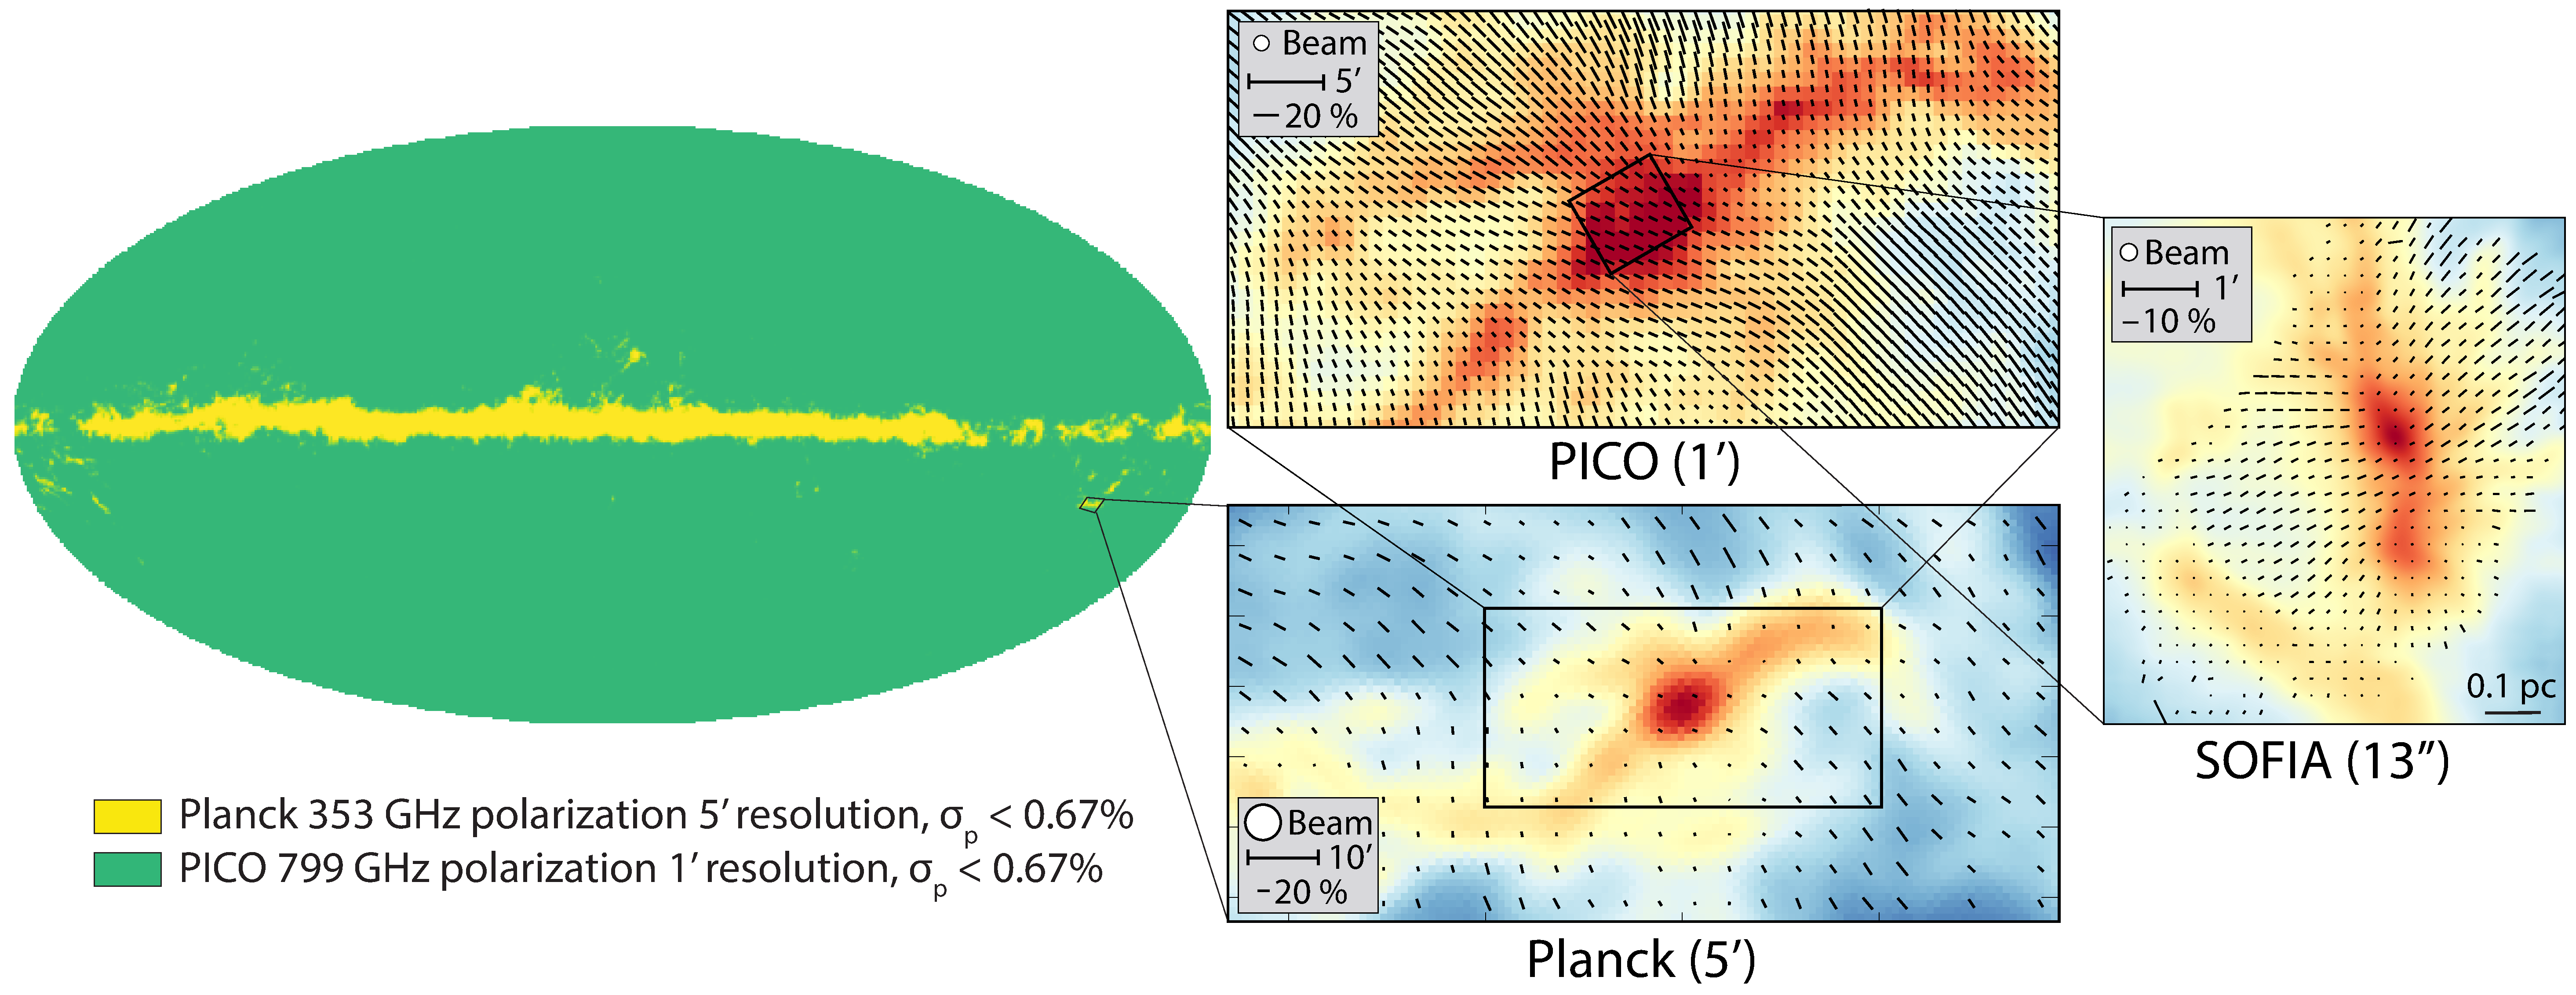
\includegraphics[width=6.5in]{images/galsci_fig_v4.pdf}
    \caption{\captiontext  \planck 's 353~GHz polarization map gave a resolution of 5\arcmin~and sensitivity to polarization intensity of $\sigma_{p} < 0.67\%$ over a small portion of the sky (left, yellow).  At 799 GHz, the PICO baseline mission will give a polarization map of the {\it entire sky} and with 5 times higher resolution (left, green). The \planck~map of the Orion region overlaid with vectors that are aligned with the inferred magnetic field (lower panel), and a simulated PICO observation (upper panel) illustrate the leap in information content (vector lengths are proportional to polarization fraction). With this map, and maps at many other frequencies that \planck~did not have, PICO will characterize Galactic magnetized turbulence at scales spanning the diffuse ISM down to dense star forming cores, which will be mapped with high-resolution polarimetry by instruments such as HAWC+/SOFIA \citep{Chuss2018} (right panel).}
    \label{fig:allsky}
\end{figure}

\noindent{\bf (1) Test Composition Models of Interstellar Dust} \\
Strong extinction features at 9.7 and 18~$\mu$m indicate that much of interstellar dust is in the form of amorphous silicates, while features at 2175\,\AA, 3.3~$\mu$m, and 3.4~$\mu$m attest to abundant hydrocarbons. It is unknown, however, whether the silicate and carbonaceous materials coexist on the same grains or whether grains of each composition grow through distinct, parallel pathways dictated by their surface chemistry. 
%If there are indeed multiple grain populations, this will induce additional challenges for modeling the emission from interstellar dust in both total intensity and polarization at levels relevant for B-mode science at all angular scales~\citep{Hensley2018}. 

%\comor{The last sentence implies that the issue of multiple grain populations is only important for CMB B-mode science. Is it? Is it not important on its own right, because it is important to know what dust is made of? This is the missing connection to the broader picture: why do we care about dust?}

Some data suggest that the populations are distinct. Spectropolarimetry of dust extinction reveals robust polarization in the 9.7\,$\mu$m silicate feature~\citep[e.g.,][]{Smith2000}, indicating that the silicate grains are aligned with the interstellar magnetic field. In contrast, searches for polarization in the 3.4\,$\mu$m carbonaceous feature have yielded only upper limits, even along sightlines where silicate polarization is observed~\citep{Chiar2006,Mason2007}. These data are consistent with silicate and carbonaceous materials existing on separate grains that have different alignment properties. 
%\comblue{However, the 3.4~$\mu$m feature arises only from aliphatic (chain-like) carbonaceous material, which may not trace all carbon-bearing grains. Additionally, available data are restricted to only a few highly-extincted sightlines that may not typify the entire diffuse \ac{ISM}.}

At odds with the spectropolarimetric evidence from dust extinction are current measurements of the polarization fraction of the far-infrared dust emission with \planck~\citep{Planck_Int_XXII} and BLASTPol~\citep{Ashton2018}. They show little to no frequency dependence, whereas substantial frequency dependence would be expected if two components with distinct polarization properties were contributing to the total emission. 
%\comblue{However, current uncertainties are relatively large and the BLASTPol data are from only high density sightlines that may not be representative of the diffuse \ac{ISM}. }

With excellent polarization sensitivity, even in diffuse regions, PICO will provide a definitive test of the two component paradigm \citep{Meisner2015}. 
%\comblue{To assess PICO's ability to discriminate models quantitatively, we employed the analytic two component dust model of Meisner et al.~\cite{Meisner2015}, which provided a better fit to IRAS and \planck\ data than one component models. We ran 1000 simulations with different combinations of polarization fractions of the two components. We used PICO baseline noise levels, frequency bands at and above 107~GHz, and binned the simulated data in 7.9$^\prime$ pixels, matching the beam of the PICO 107~GHz band.} 
If there are two dust components, the PICO baseline mission will determine the intrinsic polarization fractions of the two components to a precision of 0.03. The data will therefore validate or reject state-of-the-art dust models~\citep[e.g.][Hensley \& Draine, in prep]{Guillet2018}, test for the presence of additional grain species with distinct polarization signatures, such as magnetic nanoparticles~\citep{Draine2013}, and will be used as a crucial input for the foreground separation necessary to extract cosmological B-mode science . %
%
%\comor{perhaps here talk about B-mode foregrounds and connect to AME?}
%\comor{give a sentence about AME: An additional emission of unknown origin has been detected in ... GHz. It is called AME ... The \ac{AME} is an important foreground in the 20-60~GHz region, but at this time the level of polarization of the AME remains controversial~\cite{Dickinson2018b}, and the spectral profile has only been well-characterized in very bright regions. } 

``Anomalous Microwave Emission (AME)'' is a component of Galactic emission peaking in the 20-30~GHz range that has been tentatively identified with small, rapidly-spinning dust grains.\citep{dickinson/etal:2018} As only upper limits have been placed on its polarization, its role as a foreground for B-mode science remains unclear. Given the present uncertainty on its physical origin and SED variability, even small levels of polarization could prove challenging. However, PICO will finely sample the AME SED with its bands at 21, 25, 30, 36, and 43 GHz. Combined with ground-based maps at lower frequencies \citep[e.g., C-BASS][at 5~GHz]{Dickinson2018a}, PICO will efficiently separate the AME from synchrotron and free-free emission and either detect or place stringent upper limits on its polarization.
%the PICO data set will utilize the distinct spectral dependence of synchrotron ($I_{\nu} \propto {\nu}^{-1}$), free-free ($I_{\nu} \propto {\nu}^{-0.1}$), and \ac{AME} to enable reliable component separation. 
Further, the enhanced frequency coverage will enable characterization of systematic changes in the AME SED with interstellar environment and thus elucidate its underlying physics.

\noindent{\bf (2) Determine how magnetic fields affect the processes of molecular cloud and star formation} \\
Stars form out of dense, gravitationally unstable regions within molecular gas clouds, which themselves form through the flow of diffuse, atomic-phase gas to denser regions. Magnetic fields play an important role throughout this process. 

On the largest scales, magnetized turbulence mediates the flow of the gaseous \ac{ISM} from the atomic to the denser, molecular phase. Recent observations suggest that the structure of the diffuse medium is highly anisotropic, and strongly coupled to the local magnetic field~\citep{Clark:2014, Clark:2015, Kalberla:2016, KalberlaKerp:2016}. 
As molecular gas clouds collapse to form stars, magnetic fields can slow the process of star formation by inhibiting movement of gas in the direction perpendicular to the field lines. Observations to date suggest that the outer envelopes of clouds can be supported against gravity by magnetic fields and turbulence, but in dense cores gravity tends to dominate, and so these dense structures can collapse to form stars \citep{Crutcher2010}.  The degree to which magnetic fields affect the formation of molecular clouds, as well as stars within these clouds,  is poorly constrained, in large part due to the difficulty of making detailed maps of magnetic fields in the ISM.

%Stars form out of dense, gravitationally unstable regions within molecular gas clouds. The efficiency of this conversion from molecular gas to stars is very low, due to regulation from supersonic turbulent gas motions, magnetic fields, and feedback from young stars \citep{McKee2007}.  Magnetic fields may play an important role in slowing the process of star formation by inhibiting movement of gas in the direction perpendicular to the field lines.  Observations to date suggest that the outer envelopes of clouds can be supported against gravity by magnetic fields and turbulence, but in dense cores gravity tends to dominate, and so these dense structures can collapse to form stars \citep{Crutcher2010}.

%On larger scales, the formation of gravitationally unstable clouds is regulated by the flow of diffuse material into the molecular phase\comor{(?)}, a process that is mediated by magnetized turbulence in the low-density \ac{ISM}. Structure formation in the diffuse \ac{ISM} is poorly understood, but as a precursor to star formation it is crucial to understand what drives molecular cloud formation. Recent observations suggest that the structure of the diffuse medium is highly anisotropic, and strongly coupled to the local magnetic field~\citep{Clark:2014, Clark:2015, Kalberla:2016, KalberlaKerp:2016}. However, the degree to which magnetic fields affect the formation of molecular clouds, as well as stars within these clouds, is poorly constrained, in large part due to the difficulty of making detailed maps of magnetic fields in the interstellar medium.

\noindent$\bullet$ {\bf Formation of Magnetized Molecular Clouds from the Diffuse Interstellar Medium} \hspace{0.1in}
A comprehensive understanding of the magnetized diffuse \ac{ISM} is challenging because of its diverse composition, its sheer expanse, and the multi-scale nature of the physics that shapes it. To understand how matter and energy are exchanged between the diffuse and dense media, it is essential to measure the properties of the magnetic field over many orders of magnitude \comor{how many?} in column density. PICO is unique in its ability to provide the necessary data. \textit{Planck} achieved measurements of the diffuse sky at 60\arcmin\ resolution, resulting in about 30,000 independent measurements of the magnetic field direction.  With 1.1\arcmin~resolution, PICO will expand the number of independent polarization measurements to about 86,000,000. The data will thus robustly characterize turbulent properties like the Alfv\'{e}n Mach number, $\mathcal{M}_A$, across a previously unexplored regime of parameter space. 

PICO's observations will complement recently completed high-dynamic-range neutral hydrogen surveys, such as \HI4PI \citep{HI4PI:2016} and GALFA-\hi \citep{Peek:2018}, as well as planned surveys of interstellar gas, most prominently with the Square Kilometer Array (SKA) and its pathfinders. One of the open questions in diffuse structure formation is how gas flows within and between phases of the \ac{ISM}. A planned all-sky absorption line survey with the forthcoming SKA-1 will increase the number of measurements of the \ac{ISM} gas temperature by several orders of magnitude~\citep{McClure-Griffiths2015}. Quantitative comparisons of the \ac{ISM} temperature distribution from SKA-1 and estimates of the magnetic field strength and coherence length scale from PICO will elucidate the role of the magnetic field in \ac{ISM} phase transitions.
\comor{should we say: 'will elucidate the role of magnetized turbulence in the flow of the \ac{ISM} from the diffuse, atomic to the denser, molecular phase', to connect to the paragraph above?}

\noindent$\bullet$ {\bf Formation of Stars within Magnetized Molecular Clouds} \hspace{0.1in}
The role of magnetic field in star-formation is quantified by the ratio of energy stored in magnetic and gravitational fields, and the ratio of energy stored in magnetic field and that stored in turbulence. The first ratio is parameterized through a mass-to-flux ratio $\mu$, and the second
through $\mathcal{M}_A$. 

With full-sky coverage and a resolution of 1.1\arcmin, PICO will map all molecular clouds with better than 1\,pc resolution, out to a distance of 3.4\,kpc.  Extrapolating from the Bolocam Galactic Plane Survey \citep[BGPS,][]{EllsworthBowers2015}, PICO is expected to make highly detailed magnetic field maps of over 2,000 molecular clouds with thousands to hundreds of thousands of independent polarization measurements per cloud. These are the {\it only foreseeable} measurements that will give $\mu$ and $\mathcal{M}_A$ over a statistically significant sample of molecular clouds. \planck , for example, mapped only 10 nearby clouds to a similar level of detail~\citep{Planck:XXXV}. A large sample of clouds is crucial because (1) dust polarization observations are only sensitive to the magnetic field projected on the plane of the sky, and therefore polarization maps will look very different for molecular clouds observed at different viewing angles; and (2) the relative importance of the magnetic field will likely be a function of cloud age and mass. By observing thousands of molecular clouds PICO will determine $\mu$ and  $\mathcal{M}_A$ for different sub-classes of cloud age and mass. 

%To constrain $\mu$ and $\mathcal{M}_A$ we will apply a series of established polarization analysis techniques:
%(1) characterizing the relative orientation of cloud structures and the magnetic field \citep{Soler2013,Chen2016,Soler2017,Planck:XXXV}; (2) making probability distributions functions of polarization measurables \citep{Fissel2016, King2018}; (3) comparing the magnetic field and velocity gradient directions \citep{GonzalezCasanova2017,Yuen2017,Lazarian2018}; and (4) measuring the angular dispersion of the magnetic field  \citep{Davis1951,Chandrasekhar1953, Hildebrand2009,Houde2009}.
%By applying all four techniques to both PICO observations and synthetic polarization maps made from ``observing'' numerical simulations of star formation, we will quantitatively compare theory and observations. PICO's large number of frequency bands will be used to better model the temperature and polarization efficiency of the cloud dust  \citep{Andersson2015}, which can then be used to generate more realistic generation of synthetic observations from simulations for comparison with PICO observations \citep{Seifried2018}. We can then compare the observed magnetization levels derived from the PICO observations to the levels of turbulence derived from molecular gas surveys~\cite{EllsworthBowers2015, Miville-Deschenes2017}, and the efficiency of star formation, measured from near and far-IR observations of dense cores and protostars with {\em Herschel}, {\em Spitzer}, and {\em WISE}. \comor{Why italics? Tim, Qi - please check for uniformity}

%{\em PICO's ability to map thousands of clouds is not possible with any other current or proposed polarimeter}. {\em Planck}, for example, was only able to map 10 nearby clouds to a similar level of detail \citep{Planck:XXXV}. This large sample of clouds is crucial because dust polarization observations are sensitive to only the magnetic field projected on the plane of the sky, and therefore polarization maps will look very different for molecular clouds observed at different viewing angles.  {\em By observing thousands of molecular clouds PICO will determine the role of magnetic fields in star formation as a function of cloud age and mass.}

%
\noindent{\bf Galactic Legacy Science}\\
PICO will also produce legacy data sets that will revolutionize our understanding of how magnetic fields influence physical processes ranging from planet formation to galaxy evolution.  For 10 nearby clouds, which have distances of less than 500 pc, PICO will resolve magnetic fields on scales of 0.1~pc. This is the scale of dense cores and filaments for these clouds, and thus the observations will constrain how magnetic fields on these scales influence the formation of cloud cores.  By comparing the orientation of the core-scale magnetic fields with the orientation and sizes of proto-planetary disks, PICO will probe whether magnetic breaking influences the growth of such disks~\citep{allen_2003,li_2014}. \comor{isn't ALMA or other instruments better suited for this?}

PICO's tens of millions of independent measurements of magnetic field orientation over the entire Galaxy will probe magnetized turbulence and study how magnetic fields are generated through a combination of turbulence and large-scale gas motions \citep{Xu_2018}\comor{that has already been said before, no?}.   Key processes in the diffuse ISM, including heat transport \citep{Lazarian:2006}, streaming of cosmic rays \citep{Lazarian:2016}, and magnetic reconnection \citep{Lazarian_Vishniac:1999} are strongly dependent on the level of magnetization. \comor{Not clear what this sentence says}

Finally, PICO observations will create detailed magnetic field maps of approximately 70 nearby galaxies, with more than 100 measurements of magnetic field directions per galaxy. These observations will determine how interaction between large-scale magnetic fields, turbulence, and feedback from previous generations of star formation affects galaxy evolution and star-formation efficiency.

%\bibliographystyle{aasjournal}
%\bibliography{galsci.bib}

\end{document}

%\begin{figure}[!htb]
%\centering
%
\includegraphics[width=4cm]{images/example}
%\caption{example}
%\label{fig:im_3}
%\end{figure}
